\clearpage
\slidetitle{Conversion en vecteur}

\begin{slide} 

\begin{itemize}

	\item On peut se contenter d'aplanir la matrice des pixels de l'image, mais vecteur trop grand.
	
	\item \textbf{Autre méthode:} placer une grille sur l'image, calculer la \textit{proportion} de pixels noirs dans chaque zone, aplanir la nouvelle matrice obtenue.

\end{itemize}	

\begin{figure}[h!]
	\centering
	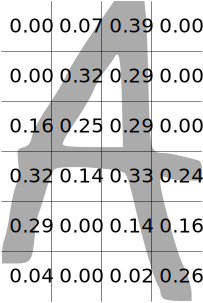
\includegraphics[width=6cm]{schemas/vectorisation.pdf}
\end{figure}

\end{slide}